\vspace{-0.1in}
\section{Introduction}
\label{sec:intro}

% \figgray{\bm{$z_s$}}


\begin{figure}
    \centering
    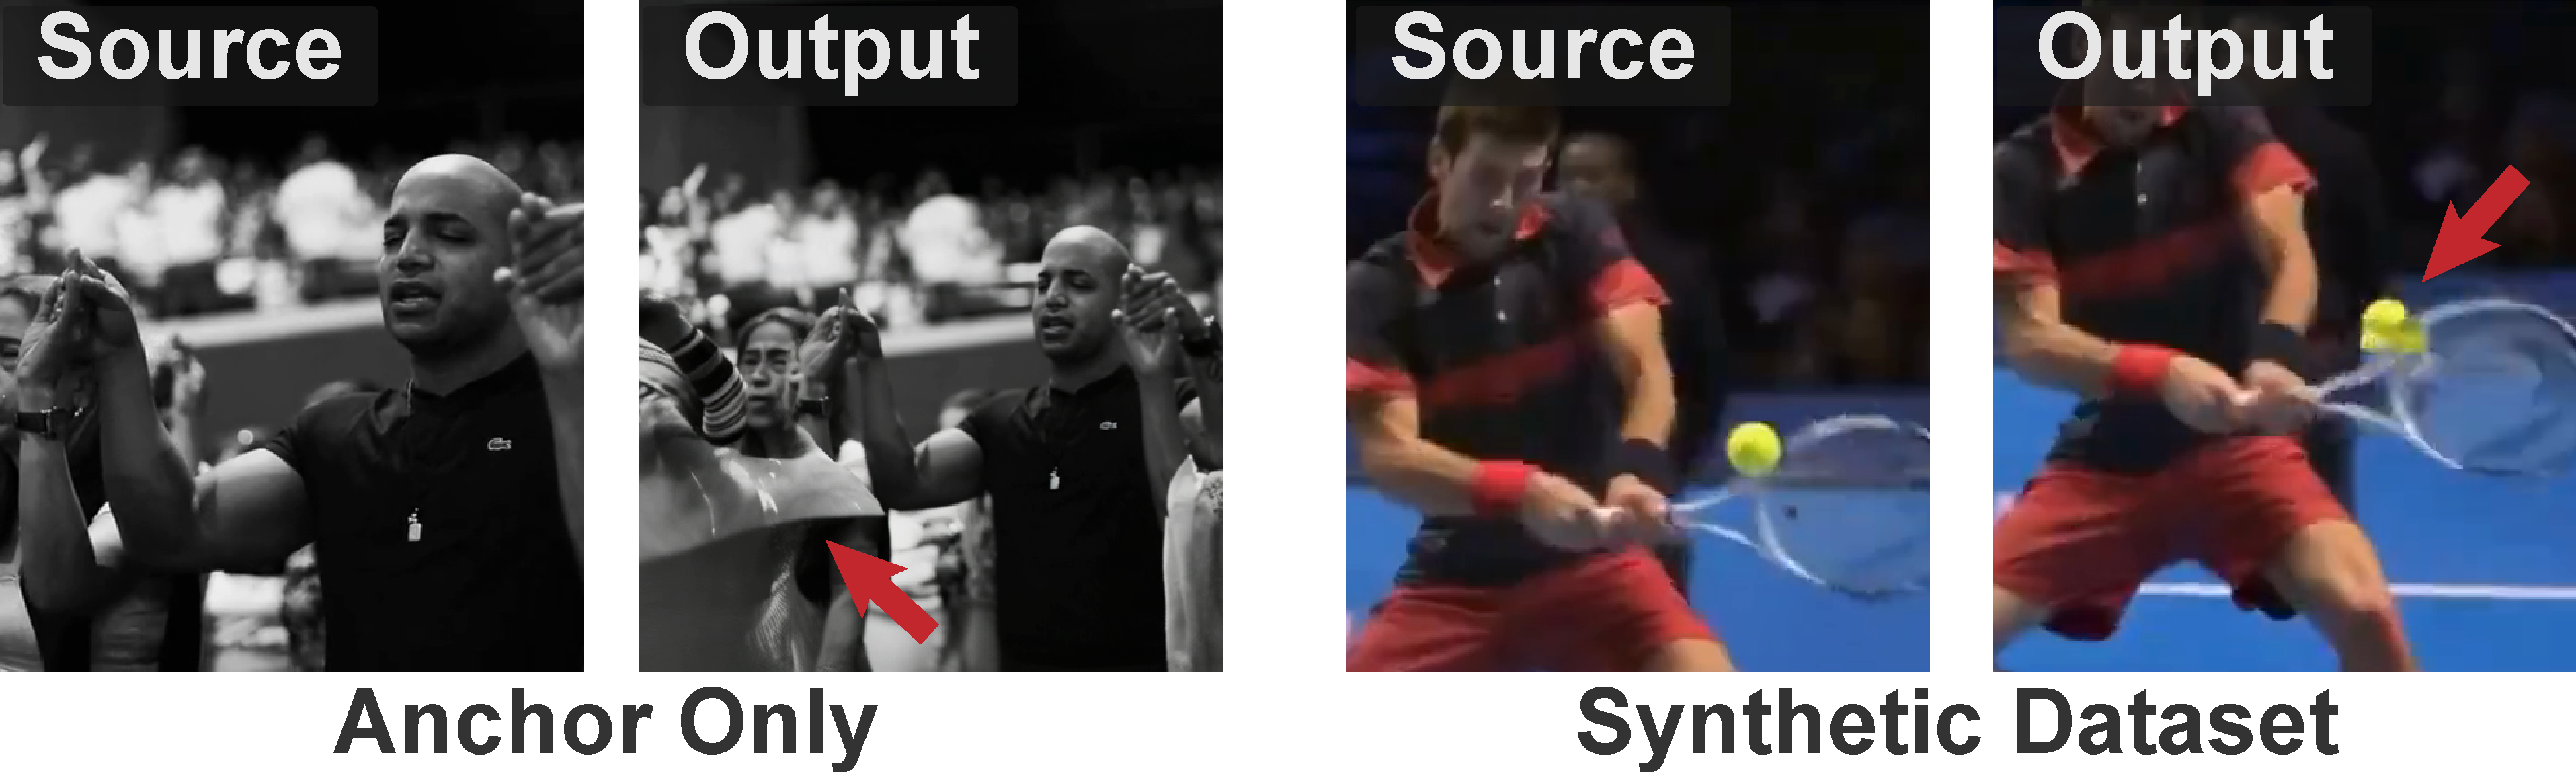
\includegraphics[width=\linewidth]{figures/motivation.pdf}
    \vspace{-0.25in}
    \caption{A comparison of video reshooting challenges. (a) Anchor-only methods~\cite{ex4d} are prone to artifacts when the anchor video $V_a$ is of low quality. (b) Synthetic data trained models~\cite{bai2025recammaster} can fail to generalize and may produce artifacts on unseen interactions, like a tennis ball being hit.}
    \label{fig:motivation}
    \vspace{-0.25in}
\end{figure}



Precise camera movement in cinematography is essential to set the scene for storytelling and to bootstrap multiple views in synthetic video generation. Digital video reshooting offers an accessible and powerful solution to digitally modify camera trajectories in post-production, as well as to improve model generalization in tasks, such as robotics, by expanding the range of training videos. 

However, developing robust video reshooting models for dynamic, non-rigid scenes is severely bottlenecked by the lack of large-scale, paired multi-view video data. To effectively train a video-to-video reshooting model, one inherently needs a pair of videos capturing the exact same action from different camera perspectives. To circumvent this scarcity, most existing approaches fall into two categories. First, some methods rely purely on large-scale synthetic datasets~\cite{bai2025recammaster, gcd}. While useful, the synthetic-to-real generalization gap is notoriously difficult to bridge. A model trained on rendered graphics struggles to generalize to the diverse domains of photorealistic video, animation, or complex dynamic interactions not seen in the training distribution, often producing significant visual artifacts (Fig.~\ref{fig:motivation}b).

Second, other methods attempt to build complex 4D representations from pretrained 3D/4D models~\cite{4d_recon_harley2025alltracker,4d_recon_hu2025depthcrafter,4d_recon_wang2024dust3r}. The simplest of these operate as \textit{anchor-only models}~\cite{ex4d}. As shown in Fig.~\ref{fig:motivation}(a), this approach is highly vulnerable to errors in the 3D/4D reconstruction, propagating artifacts in the anchor directly to the final output. Advanced techniques like \trajectorycrafter{}~\cite{yu2025trajectorycrafter} attempt to mitigate these artifacts by using the original source video as an additional input. However, these approaches remain constrained by the limited quality and high computational cost of their underlying 4D data pipelines.

In this paper, we propose a fundamentally different approach. Our core idea is a highly scalable, self-supervised strategy that generates a \textit{pseudo multi-view training triplet} (consisting of a source, anchor, and target video) from a single monocular video.

During training, we extract two distinct clips to serve as the source and target videos using smooth random walk trajectories that simulate dynamic camera motion, as shown in Fig.~\ref{fig:teaser}. We then synthetically generate the anchor video by forward-warping the first frame of the source video using a dense 2D tracker. This effectively simulates the distorted point-cloud-based inputs expected at inference. 

During inference, we convert the source video to a 4D point cloud, modify the perspective given a novel camera trajectory, and create an inference-time anchor video as geometric conditioning. The model must then predict a new target video given the anchor and the source videos.

Our training setup forces the base video model to learn a robust, 4D-aware understanding of scene dynamics. To reconstruct the target video, the model must learn to ignore reconstruction artifacts in the anchor and retrieve the correct texture from the source video. Because our cropping strategy introduces spatial misalignment and artificial occlusion, the model cannot simply copy the corresponding source frame. To fill dis-occluded regions, it is compelled to find the missing texture in a different temporal context within the source (Fig.~\ref{fig:teaser}). This spatial bottleneck acts as an information erasure mechanism, forcing the model to build an implicit 4D world prior by routing and re-projecting content across different times and pseudo-viewpoints.

Our contributions are three-fold:
\begin{itemize}[noitemsep, topsep=0pt, partopsep=0pt]
    \item First, we introduce a highly scalable, domain-agnostic self-supervised data pipeline that generates pseudo multi-view training triplets from monocular videos.
    \item Second, we propose a minimal and efficient architectural adaptation leveraging a pre-trained video diffusion model's self-attention modules. We pair this with a set of targeted training augmentations designed to ensure robust generalization to distorted, inference-time artifacts.
    \item Third, we demonstrate through extensive experiments that our approach achieves state-of-the-art temporal consistency and camera control across a diverse set of dynamic videos, significantly advancing the capabilities of video reshooting.
\end{itemize}